%%
%% Copyright 2007, 2008, 2009 Elsevier Ltd
%%
%% This file is part of the 'Elsarticle Bundle'.
%% ---------------------------------------------
%%
%% It may be distributed under the conditions of the LaTeX Project Public
%% License, either version 1.2 of this license or (at your option) any
%% later version.  The latest version of this license is in
%%    http://www.latex-project.org/lppl.txt
%% and version 1.2 or later is part of all distributions of LaTeX
%% version 1999/12/01 or later.
%%
%% The list of all files belonging to the 'Elsarticle Bundle' is
%% given in the file `manifest.txt'.
%%

%% Template article for Elsevier's document class `elsarticle'
%% with numbered style bibliographic references
%% SP 2008/03/01
%%
%%
%%
%% $Id: elsarticle-template-num.tex 4 2009-10-24 08:22:58Z rishi $
%%
%%
\documentclass[preprint,12pt,3p]{elsarticle}

%% Use the option review to obtain double line spacing
%% \documentclass[preprint,review,12pt]{elsarticle}

%% Use the options 1p,twocolumn; 3p; 3p,twocolumn; 5p; or 5p,twocolumn
%% for a journal layout:
%% \documentclass[final,1p,times]{elsarticle}
%% \documentclass[final,1p,times,twocolumn]{elsarticle}
%% \documentclass[final,3p,times]{elsarticle}
%% \documentclass[final,3p,times,twocolumn]{elsarticle}
%% \documentclass[final,5p,times]{elsarticle}
%% \documentclass[final,5p,times,twocolumn]{elsarticle}

%% if you use PostScript figures in your article
%% use the graphics package for simple commands
%% \usepackage{graphics}
%% or use the graphicx package for more complicated commands
%% \usepackage{graphicx}
%% or use the epsfig package if you prefer to use the old commands
%% \usepackage{epsfig}

%% The amssymb package provides various useful mathematical symbols
\usepackage{amssymb}
\usepackage[cmex10]{amsmath}
\usepackage{mathtools}
\usepackage{blindtext}
\usepackage{graphicx}
\usepackage{chemfig}
\usepackage{textcomp}
\usepackage{listings}
\usepackage{adjustbox}
\usepackage{tablefootnote}
\usepackage{multirow}
\usepackage[version=3]{mhchem}
%\usepackage[alf,abnt-emphasize=bf]{abntex2cite}	% pacote para usar citações abnt

%% The amsthm package provides extended theorem environments
%% \usepackage{amsthm}

%% The lineno packages adds line numbers. Start line numbering with
%% \begin{linenumbers}, end it with \end{linenumbers}. Or switch it on
%% for the whole article with \linenumbers after \end{frontmatter}.
%% \usepackage{lineno}

%% natbib.sty is loaded by default. However, natbib options can be
%% provided with \biboptions{...} command. Following options are
%% valid:

%%   round  -  round parentheses are used (default)
%%   square -  square brackets are used   [option]
%%   curly  -  curly braces are used      {option}
%%   angle  -  angle brackets are used    <option>
%%   semicolon  -  multiple citations separated by semi-colon
%%   colon  - same as semicolon, an earlier confusion
%%   comma  -  separated by comma
%%   numbers-  selects numerical citations
%%   super  -  numerical citations as superscripts
%%   sort   -  sorts multiple citations according to order in ref. list
%%   sort&compress   -  like sort, but also compresses numerical citations
%%   compress - compresses without sorting
%%
%% \biboptions{comma,round}

% \biboptions{}

\lstset{language=C++,
	basicstyle=\ttfamily\scriptsize,
	keywordstyle=\color{blue}\ttfamily,
	stringstyle=\color{red}\ttfamily,
	commentstyle=\color{green}\ttfamily,
	breaklines=true}
	
\renewcommand{\lstlistingname}{Code}


\journal{Simulation modeling Practice and Theory}
% http://www.journals.elsevier.com/simulation-modeling-practice-and-theory/
\begin{document}

\begin{frontmatter}

\title{\emph{SHPECK} - A Geochemical Speciation Modeling Software}
%\title{SHPECK -A Computational Approach for Geochemical modeling Speciation: Chemical Equilibrium Calculation}

\author[label1]{Leonardo Hax Damiani\corref{cor1}}
\address[label1]{Institute of Informatics, UFRGS, Porto Alegre, RS, Brazil}

\cortext[cor1]{Corresponding author}

\ead{lhdamiani@inf.ufrgs.br}
\ead[url]{http://www.inf.ufrgs.br/~lhdamiani}

\author[label2]{Marcos Antonio Klunk}
\ead{marcos.klunk@ufrgs.br}
\address[label2]{Institute of Geoscience, UFRGS, Porto Alegre, RS, Brazil}

\author[label1]{Renata Galante}
\ead{galante@inf.ufrgs.br}

\author[label1]{Mara Abel}
\ead{mara@inf.ufrgs.br}

\author[label3]{Anthony Jung Park}
\ead{ajpark@sienna-geo.com}
\address[label3]{Sienna Geodynamics, Albany, NY, USA}

\author[label1]{Carla Maria Dal Sasso Freitas}
\ead{carla@inf.ufrgs.br}

\begin{abstract}
Geochemical speciation modeling software are used for calculating the distribution of dissolved solute and complex compound species in water, and also to compute saturation indices of minerals. In this work we introduce \emph{SHPECK}, a software developed to model geochemical speciation using the mass-balance conditions and the phase rule \cite{Garrels:65}. SHPECK can be used to model the chemical equilibrium interaction between elements and solutes. It provides an interactive and intuitive user interface, as well as the support of a relational database structure that handles the management of thermodynamic and material properties data used for the geochemical modeling. We review the available geochemical modeling software (only programs that provide speciation modeling), highlighting relevant characteristics as: input and output options; user interaction; file formats; and software environment and installation procedure. The software \emph{SHPECK} is validated by modeling the diagenetic reactions observed in a siliciclastic geological system, and by performing a comparative study with other modeling software packages. In addition to this, a database comparison was addressed and the results demonstrate a substantial improvement on the performance by the use of the \emph{SHPECK}'s relational database comparing to the existing approaches.
\end{abstract}

\begin{keyword}
%% keywords here, in the form: keyword \sep keyword
Geochemical modeling \sep
Chemical Equilibrium \sep
Geochemistry \sep 
Multiphase System \sep
Law of Mass-Action \sep
Nonlinear simulation \sep
Software Engineering \sep
Computational simulation \sep

%% MSC codes here, in the form: \MSC code \sep code
%% or \MSC[2008] code \sep code (2000 is the default)
\end{keyword}

\end{frontmatter}

%%
%% Start line numbering here if you want
%%
% \linenumbers

%% main text
\section{Introduction}
Geochemical speciation modeling describes the process of simulating chemical reactions that occur between the water (solvent) and chemical elements. The motivation of this study is to provide a better understanding of the diagenetic process occurring in sediments, especially the water-mineral chemical interaction. Applications of geochemical models are essential in several environmental problems, such as calculating compositions of natural ground or surface waters, and precipitation and/or dissolution of minerals. A geochemical speciation modeling software is responsible for calculating the distribution of dissolved species into solutes and aqueous complexes, and also for computing saturation indexes for different mineral. 

In this work, we present the software system \emph{SHPECK} that allows simulations of chemical equilibrium reactions occurring in geochemical systems using the mass-balance approach and the phase rule as described in Garrels and Christ \cite{Garrels:65}. The software system receives as input any general combination of chemical elements, species, and reactions, allowing the user to create several different environments, simulations and, therefore, to fully and easily control any aspect and configuration of the model. Moreover, our work shows a thorough analysis of the available existing solutions, making clear the uniqueness of our approach for the geochemical modeling software design.

The software \emph{SHPECK} also provides an interactive user interface that allows the users to more conveniently setup the simulations. The user interface uses a relational database that further improves database access and management, which is an option absent in any of the other public-domain alternatives.  The flexibility of parameter configuration offered by the visual interface further extends the possibilities of experimentation with the software. Limitations on the database structure and input capability strongly restrict the potential use of the alternative geochemical packages. Therefore, \emph{SHPECK} is unique among the geochemical speciation models by implementing modern computing technology, absent in other similarly tasked software, and also employing efficient numerical methods.

\section{Review of Available Geochemical modeling Software}
Geochemical modeling software have been in use since the 70’s to solve: speciation; determination of mineral saturation index; mixing of compositionally distinct  waters; calculation of stoichiometric reactions; mixing of solids, fluid and gas phases; calculation of equilibrium and kinetic reactions between solutes and minerals; and reactive transport. While a large number of computational models have been developed over the years, a number of them are particularly well known and available to general public. Thus, three models representing the large number of similar software have been identified and compared in this study: \emph{EQ3/6}, \emph{PHREEQC} and \emph{MINTEQ}. We had given special attention to the geochemical modeling approaches and the software engineering aspects adopted in their implementations, providing the comparison when the information is available. Since SHPECK is a speciation model, the reactive-transport and kinetic features available in some of the alternative models will not be addressed.

\emph{EQ3/6} consists of two programs: \emph{EQ3} is a speciation code whose results EQ6 subsequently processes. It is a software package for geochemical modeling of aqueous systems written in \emph{FORTRAN77}. \emph{EQ3/6} includes a speciation-solubility solver, which is useful for analyzing groundwater chemistry data, calculating solubility limits and determining whether certain reactions are in partial equilibrium or in state of disequilibrium. It also offers a reaction path calculation that models water/rock interaction or fluid mixtures. EQ3/6 supports several thermodynamic data files. These data files also include supports for \emph{Davies}, \emph{B-dot}, \emph{Debye Huckel} equations used to approximate activity of solutes in water, as well as data for standard-state properties of solutes. Currently available versions run under \emph{UNIX-like} environments, and the full package distribution requires a paid license. Additional details of the software can be found in \cite{Wolery:1979}, \cite{Wolery:1990} and \cite{Wolery:1992}.

\emph{PHREEQC} stands for \emph{PH} \emph{RE}dox \emph{EQ}uilibrium in \emph{C} language, and is largely used geo chemical modeling software obtainable from the \emph{USGS}. Versions for Windows and UNIX-like operating systems are available. A detailed description of the package can be found in \cite{Parkhurst:95}. It was designed to perform a wide variety of low-temperature aqueous geochemical calculations based on an ion association aqueous model. It includes functionality for:
\begin{itemize}
\item Speciation and Saturation Index calculations;
\item Batch reaction and one-dimensional (1D) transport calculations involving reversible reactions (including aqueous, minerals, gas, solid-solution, surface-complexation, and ion-exchange equilibrium) and irreversible reactions (including specified mole transfer of reactants, kinetically controlled reactions, mixing of solutions and temperature changes);
\item Inverse modeling, which finds sets of mineral and gas mole transfers that takes into account differences in water composition.
\end{itemize}

\emph{MINTEQ} \cite{Felmy:84}  is a geochemical program for modeling aqueous solutions and their interactions with hypothesized assemblages of solid phases. It has a particular inclination for calculating equilibrium composition of dilute aqueous solutions. The model is useful for calculating the equilibrium mass distribution among dissolved species, adsorbed species and multiple solid phases, limited by a simple treatment of the reactions. It was originally developed in \emph{FORTRAN77} by the \emph{Battelle Pacific Northwest Laboratories} (\emph{BPNL}) and continues to be maintained by the \emph{Environmental Protection Agency} (\emph{EPA}) to perform the necessary calculations regarding waste, sediments and ground water interaction. \emph{MINTEQ} does not consider the kinetic reactions and works at fixed temperature ($25$ degrees Celcius). An extensive database is included in the software \cite{Brown:87} \cite{Allison:91}. 
The latest update on \emph{MINTEQ} dates from 1990. Limited improvements on the usability and calculations have been added since, and the new version is named \emph{MINTEQA2}. The new version supports the thermodynamic database from the \emph{USGS}. In this article only the \emph{MINTEQA2} is reviewed.

\subsection{Input and Output Format}
\emph{EQ3/6} and \emph{MINTEQA2} work with more than one input files, that are generated manually and given to the program as arguments. It is important to note that they must be mutually consistent with the options and methods chosen. Wrong chemical data or inconsistencies in the chosen algorithm will lead to erroneous results. \emph{PHREEQC} uses the same approach, however a visual plugin \cite{NotPhree:11} and a \emph{GUI} \cite{pfw:11} make it possible to reduce the error. It is often very tedious and time consuming to generate input files for simulations. Output formats of the three software systems are similar: text files with blocks of information reporting input options, variables and results of the simulations.

\subsection{User Interaction}
\emph{EQ3/6}, \emph{MINTEQA2} and \emph{PHREEQC} (\emph{UNIX-like} distribution) establish all interactions with users through command lines, since there are no graphical interfaces. Once the simulation process starts, any change in the parameters requires to kill the process manually through the operating system and run the simulator again. The \emph{PHREEQC} package provides a version for Windows \cite{pfw:11}, however it has not been updated since 2011. This version allows the user to generate input files, however there are no error verification or analysis capabilities.

\subsection{File formats}
All three software mentioned work with text input files (\emph{ASCII}), which can be created and edited using any text editor.

\subsection{Thermodynamic database}
The three software use flat files as thermodynamic database. This procedure has several potential issues: duplication of the information; non-unique records; difficulty updating and maintaining; inherently inefficient; rigid (difficult data format); and insecure \cite{dauerer2000system}.

\subsection{Software environment and installation procedures}
\emph{EQ3/6} has no self-extracting installer, and the installation process requires some level of proficiency with command prompts and \emph{DOS}. Furthermore, \emph{EQ3/6} is available only for \emph{Windows}; the \emph{UNIX} distribution is no longer available. \emph{PHREEQC} and \emph{MINTEQA2} have \emph{Windows} installers available for download.  \emph{MINTEQA2} distribution on \emph{UNIX} environment consists of the source code, thus requiring the user to compile and link.
\emph{EQ3/6} and \emph{MINTEQA2} were written in \emph{FORTRAN77} while \emph{PHREEQC} is written in \emph{C}.

\section{SHPECK}
\emph{SHPECK} is a geochemical speciation modeling software capable of calculating the distribution of dissolved species between free ions and aqueous complexes and also the saturation indices for different mineral. \emph{SHPECK} was developed using \emph{C++} and is modelled following the concept of \emph{Model-View-Controller} (\emph{MVC}) \cite{Gamma:94}. The architecture is presented in figure~\ref{fig:shpeck-architecture}.

\begin{figure}[ht!]
\centering
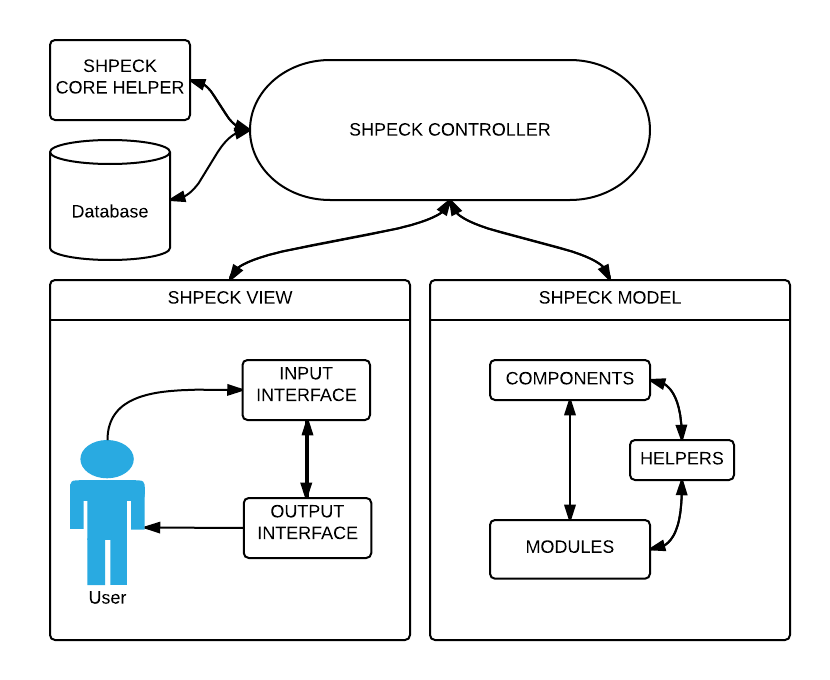
\includegraphics[width=100mm]{shpeck-architecture.png}
\caption{Architecture of the \emph{SHPECK} software}
\label{fig:shpeck-architecture}
\end{figure}

Figure~\ref{fig:shpeck-architecture} shows the three interconnected architecture components of the \emph{MVC} architectural pattern:		
\begin{itemize}		
\item Model: It encompasses the algorithms and math needed for computing the state of the system at each time step. For example, the computation of the activity coefficient using the Debye-Hueckle's formula. 
\item View: It provides all the visualization of the state of the model. For example, the solutes that the user wants to add into the chemical composition of the water.		
\item Controller: It comprises the methods to change the model's state. For example, define how to calculate the activity coefficient according to the user's choice or the value of the ionic strength.		\end{itemize}

\subsection{Graphical User Interface}
In existing geochemical modeling software systems, the \emph{GUI} are either poorly implemented, or not implemented at all. The \emph{GUI} of \emph{SHPECK} enables a user to interactively construct a geochemical system for modeling. \emph{SHPECK}'s \emph{GUI} uses tabs to address different criteria and input types:
\begin{itemize}
\item Configurations panel (figure~\ref{fig:config}): this panel allows users to view and manipulate basic system settings and to control temperature, activity coefficient calculation method, the number of iterations, solver options, and other numerical method parameters.
\item Chemical phases in the water panel (figure~\ref{fig:water}): this panel allows users to create and edit composition of waters that are used in the model. This section has access to the complete catalog of solutes database. The solutes in the tab with non-zero concentrations are included in the simulations. 
\item Results panel (figure~\ref{fig:output}): This panel allows users to examine input information and simulation results, such as temperature, ionic strength, pH of the solution, final concentration for the solutes, saturation indices, etc.
\end{itemize}

\begin{figure}[ht!]
\centering
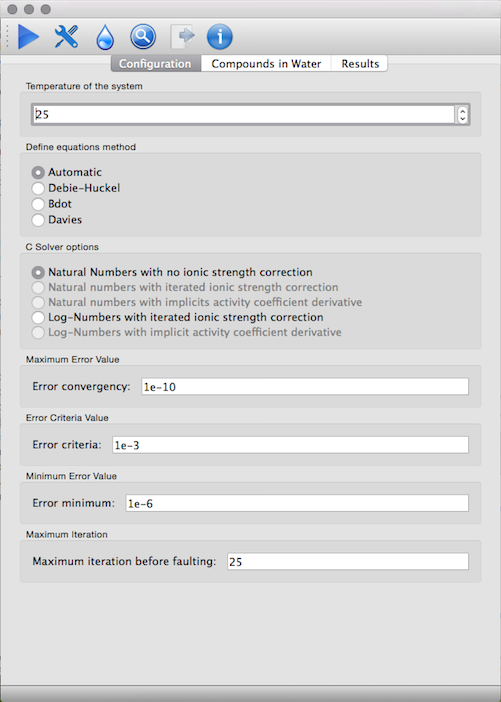
\includegraphics[width=100mm]{shpeck-configtab.png}
\caption{Configuration panel}
\label{fig:config}
\end{figure}

\begin{figure}[ht!]
\centering
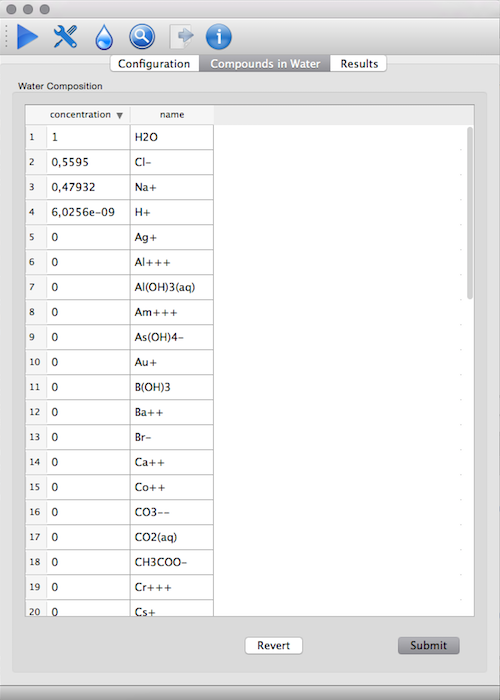
\includegraphics[width=100mm]{shpeck-watertab.png}
\caption{Water composition panel}
\label{fig:water}
\end{figure}

\begin{figure}[ht!]
\centering
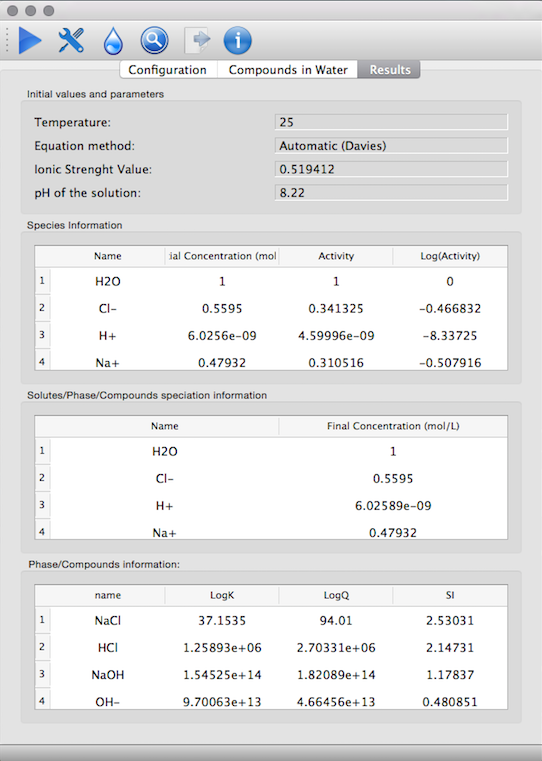
\includegraphics[width=100mm]{shpeck-resultstab.png}
\caption{Results panel}
\label{fig:output}
\end{figure}

\subsection{Database}
A relational database is used in \emph{SHPECK} to bypass the problems associated with the use of text files used as databases in other software, and to provide flexible and rapid, visually effective correlation between information required and available through the database enquiries. In addition, relational databases offer three important advantages:
\begin{itemize}
\item  Memory saving, since it does not require the complete database to be fully loaded in the main memory during the run time. The program fetches the information only when required by each module. 
\item Direct access to relevant information: SQL queries are used to fetch only the relevant information, whereas sequential search is required when text files are used. Database queries and concatenation of queries result in a faster and more efficient use of the available resources.
\end{itemize}

The database model, presented in details in figure~\ref{fig:ERDiagram}, was defined after studying the algorithm and determining what would be the structure and the information needed.  The relational database embraces all the important data required, and the structure was defined to both organize and compact the structure, thus making the information access more efficient. 

\begin{figure}[ht!]
\centering
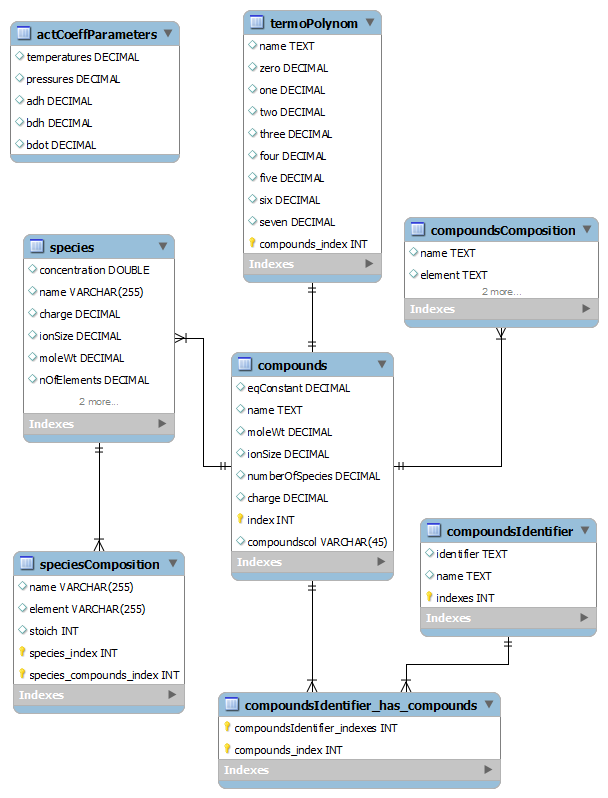
\includegraphics[width=100mm]{ER_diagram.png}
\caption{Diagram of the database}
\label{fig:ERDiagram}
\end{figure}

We adopted a \emph{SQLite} database \cite{SQLite}, which is a software library that implements a self-contained, transactional \emph{SQL} open source database engine. Currently it is the most widely deployed \emph{SQL} database engine in the world.

\emph{SHPECK}'s database is composed by the information on elements, solute species, compounds, reactions, and thermodynamic constants from the \emph{Lawrence Livermore National Laboratory} (\emph{LLNL}) thermodynamic dataset. A parser for \emph{LLNL} flat file database was created to extract this information from text files and to populate the database tables. The same text files are used as database in \emph{EQ3/6}, \emph{PHREEQC} and other geochemical codes.

Once the structure and the technology of our database were defined, a program was implemented to extract (i.e., parse) the information from the flat file database. 
The parser was generated in order to ensure that all of the data and delimiters were identified and treated properly, because of irregularities found in the flat files (i.e. wrong tab or space formatting, different encoding of the files, etc).

\section{Verification and Validation}
To test and validate the simulator, we modeled the diagenetic reactions observed in Snorre Field reservoir sandstones of Norwegian North Sea. The main reservoir horizons of the field are the fluvial sandstones in the upper member of the Upper Triassic Lunde Formation and the Upper Triassic to Lower Jurassic Statfjord Formation \cite{Hollander:87}. The sandstones sampled for this study, according to Morad \cite{Morad:90}, belong to the upper member of the Lunde Formation. The sandstones are dominantly fine- to medium-grained and arkosic with framework constituents of quartz (40-80\%), K-feldspar (5-12\%), plagioclase (15-45\%), muscovite, biotite and clay minerals. That include smectite, mixed-layer clay minerals, chlorite and subordinate amounts of kaolinite and illite. Subordinate rock fragments include intraformational mudstone and carbonate clasts and extrabasinal grains of quartz-feldspar-mica aggregates that probably represent granitic rocks and/or schist or gneisses. Mica and detrittal clay minerals seldom make up more than 2\% of the total mineral content in the sandstones. Diagenetic clay minerals include pore-filling kaolinite and pore-lining smectite, mixed-layer chlofite-smectite, and chlorite. Other cements include the carbonates (0.0-25\%) which play a significant role in porosity reduction in some of the sandstones. Authigenic overgrowths are primarily quartz, anatase and minor albite, pyrite and barite.

The descriptions presented in \cite{Morad:90} of the diagenetic reactions that take place in the Snorre Field allowed us to generate results to carry out a computationally comparative study. Morad's work describes the texture, origin, chemistry of the sandstones reservoirs in terms of the water composition and temperature. We modeled and compared the same diagenetic environment using \emph{SHPECK}, \emph{PHREEQC} and \emph{MINTEQA2}. The water composition is detailed in \cite{Nordstrom:79}.

As stated in \cite{Morad:90}, the model presented in \cite{Egeberg:88} calculates activities of the various ions of formations waters using the ion association model (originally described in \cite{Wigley:77}). The thermodynamics data used are given in \cite{Helgeson:74a},  \cite{Helgeson:74b}, \cite{Helgeson:76}, \cite{Waltter:77}, \cite{Helgeson:78} and \cite{Helgeson:81}.

The activity diagram generated for a known temperature and log activity ratio of Potassium to Sodium ions of \cite{Aagaard:90} is provided as input to \emph{SHPECK} model (Figure ~\ref{fig:tempXactratio}). The results show a consistent pattern: as the temperature rises the potassium activity becomes higher than sodium’s, which means that the phases associated to the ion potassium (i.e. K-feldspar, Illite, etc) are dissolving.


\begin{figure}[ht!]
\centering
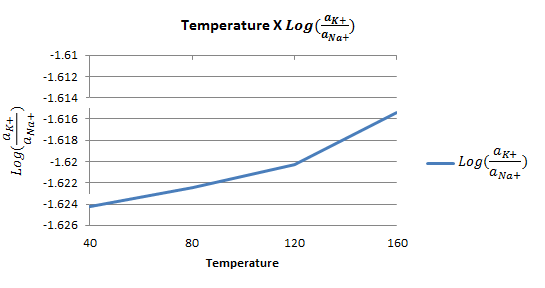
\includegraphics[width=100mm]{tempXactratio.png}
\caption{Log activity ratio of Potassium to Sodium ions using the results from \emph{SHPECK}}
\label{fig:tempXactratio}
\end{figure}

\subsection{Comparative study} 
By modeling the same environment using three distinct software packages, we attain a relevant comparison among the numerical methods and algorithms.

Chemical composition of the water adopted in the models is taken from  \cite{Nordstrom:79} which provides the chemical composition of the seawater (table ~\ref{tab:nordstrom}). The comparative study tested temperatures from $25^o$C to $100^o$C. In \emph{MINTEQA2}, due to limitations of its thermodynamics equilibrium database, the maximum temperature available is $100^o$C.

\begin{table}
\caption{Chemical composition of the solution in the sea water at $25^oC$ in $mM/L$}
\label{tab:nordstrom}
\centering
\begin{tabular}{r|c|c|c|c|c|c|c|c|c}
\ce{Al^{3+}} & \ce{K^+} & \ce{Na^+} & \ce{Ca^{2+}} & \ce{Mg^{2+}} & \ce{Fe^{2+}} & \ce{SiO_2}&  
\ce{SO_4^{2-}} & \ce{Cl^-} & pH
    \\ \hline
7.59e-5 & 10.45 & 479.32 & 10.53 & 54.39 & 3.66e-5 & 0.073 & 28.893 & 559.5 & 8.22
\end{tabular}
\end{table}

We aim to model the diagenetic processes that best represent the behavior of ions in the water-rock interactions. Figures ~\ref{fig:na+},~\ref{fig:cl-},~\ref{fig:mg+2} and ~\ref{fig:ca+2} present the most representative ions of the solution. The results of \emph{SHPECK} are similar to those from both \emph{PHREEQC} and \emph{MINTEQA2} in most of the cases, especially for temperatures under $100^o$C. Discrepancies occur in \emph{SHPECK} and \emph{PHREEQC} results when temperatures are higher than $100^o$C. This discrepancy is due to incomplete equilibrium constant \emph{K} defined in the MINTEQA2 database.

This is a known issue from \emph{LLNL} thermodynamic dataset: sometimes equilibrium constants have no measures in literature and are treated as unknowns. In such cases \emph{SHPECK} adopts the nearest equilibrium constant known value. Unfortunately we do not have access to the whole software’s details in order to describe how other software handle treat this issue.

\begin{figure}[ht!]
\centering
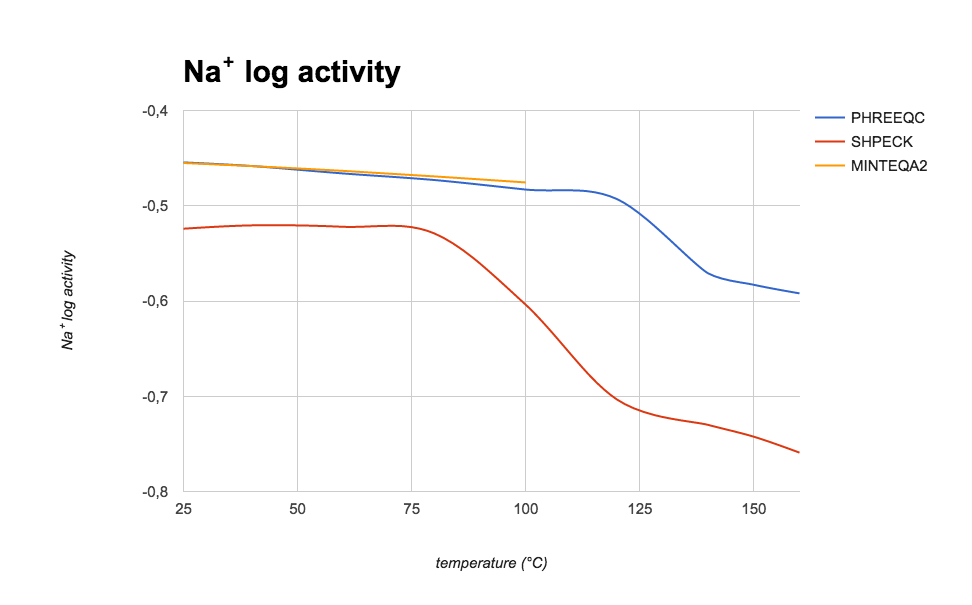
\includegraphics[width=140mm]{na+.png}
\caption{\ce{Na^+} log activity comparative study}
\label{fig:na+}
\end{figure}

\begin{figure}[ht!]
\centering
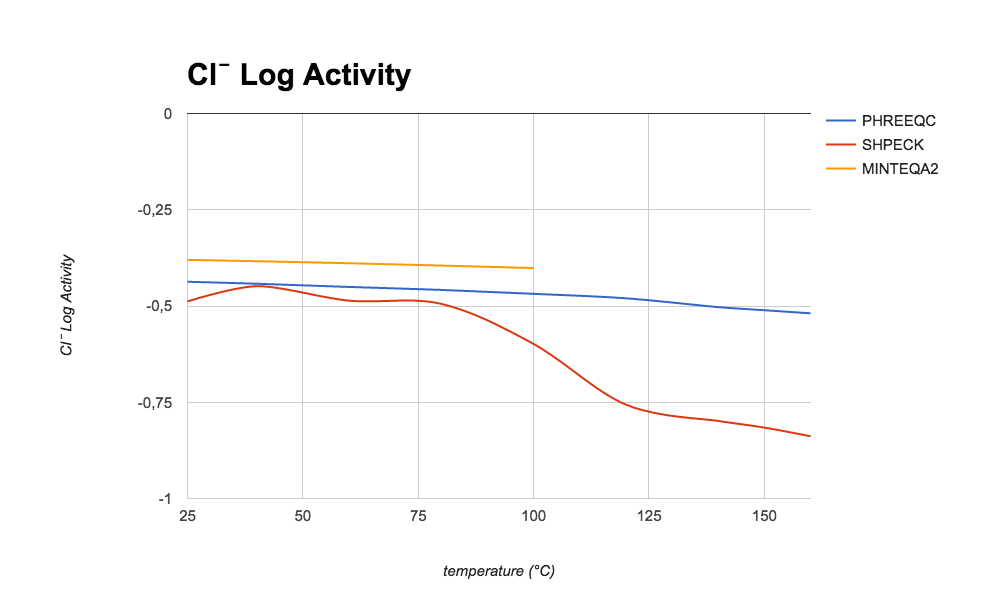
\includegraphics[width=140mm]{cl-.png}
\caption{\ce{Cl^-} log activity comparative study}
\label{fig:cl-}
\end{figure}

\begin{figure}[ht!]
\centering
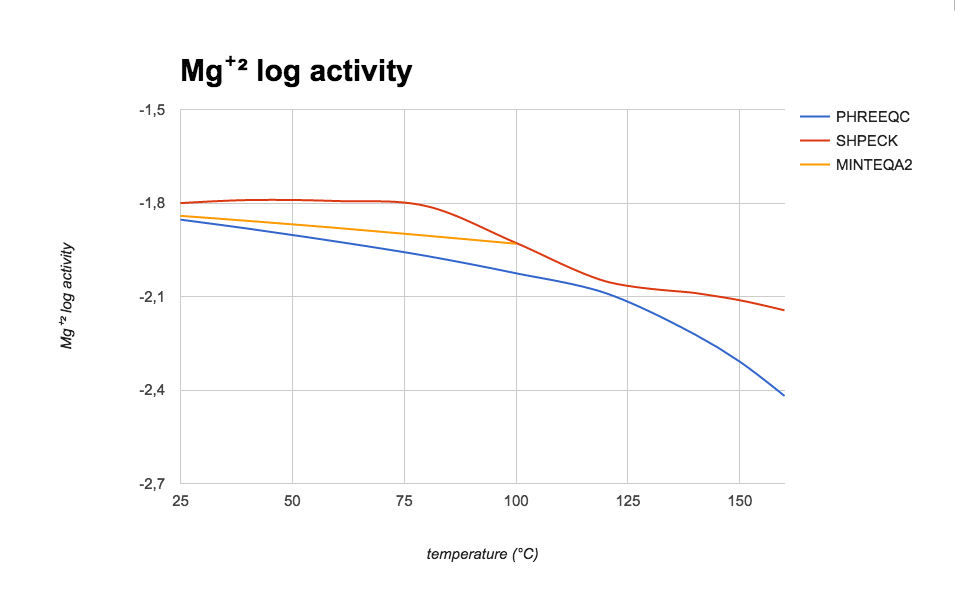
\includegraphics[width=140mm]{mg+2.png}
\caption{\ce{Mg^{+2}} log activity comparative study}
\label{fig:mg+2}
\end{figure}

\begin{figure}[ht!]
\centering
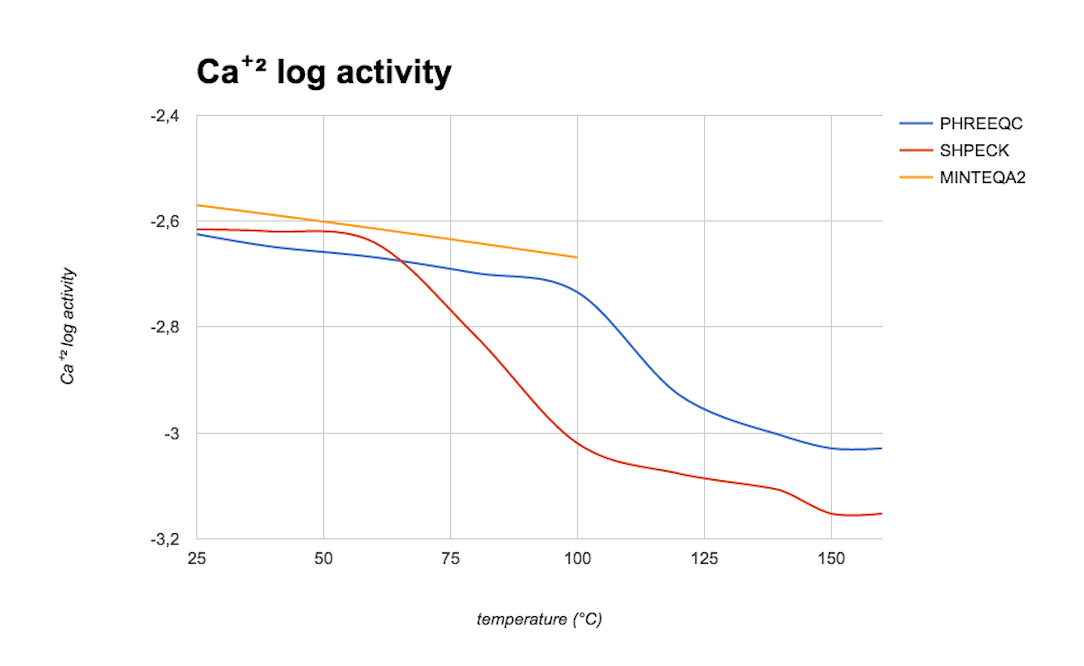
\includegraphics[width=140mm]{ca+2.png}
\caption{\ce{Ca^{+2}} log activity comparative study}
\label{fig:ca+2}
\end{figure}

\subsection{Database Evaluation}
All geochemical models used for comparison studies use text files as databases. The goal of this section is to make clear the difference and, more importantly, the benefits of \emph{SHPECK}’s relational database. Most of the information inside a geochemical database is related to each other (i.e. a mineral phase is described by a reaction, a reaction is composed by solute species, and a solute species is composed of chemical elements). Relational database’s sophisticated built-in query and sorting statements make the organization of the data convenient, and this significantly improves the performance and robustness of the application. On \emph{SQLite} databases, the data can be accessed using \emph{SQL} queries that reduce the complexity and increase the speed on information retrieval. Code~\ref{cod:sqlQuery} shows a typical query issued from \emph{SHPECK}’s \emph{SQLite} query. The options and the flexibility afforded by the use of relational database cannot be compared to the options available when textfile-based databases are used.

\begin{minipage}{0.8\linewidth}
\begin{lstlisting}[frame=single, label=cod:sqlQuery, caption=\emph{SHPECK}'s \emph{SQLite} example query]
SELECT compoundsComposition.element, compoundsComposition.name, compoundsComposition.stoich, compounds.eqConstant, termoPolynom.zero, termoPolynom.one, termoPolynom.two, termoPolynom.three, termoPolynom.four, termoPolynom.five, termoPolynom.six, termoPolynom.seven FROM termoPolynom, compoundsComposition, compounds WHERE compoundsComposition.name = compounds.name AND termoPolynom.name = compounds.name AND compounds.name = XXXXX;
\end{lstlisting}
\end{minipage}

During the model input design, the value ”XXXX” in Code 1 is updated to the simulation’s solute name. The information fetched with this query comes from three different tables, and thus, many relevant information for the simulation is fetched at once.

\subsection{Time analysis}
The response time is considered as the sum of the processing time and the time waiting for the availability of the resource. It is necessary to understand that until the software has received all the information requested from the database it is inactive and in a standby mode. To analyze the response time within a geochemical analysis point of view, we discuss not only the access time, but also the implications of that information.

When fetching any information from a thermodynamic database, it is important to take into consideration additional allied data that will also have to be retrieved. For example, when fetching a reaction data, the basic information consists of the compounds that take part in this reaction and the related stoichiometric values. Behind this action, the database must also provide information about the compounds (i.e. charge, ion size, molecular weight, elements in that species, formula, and molar volume), as well as the reaction (i.e., thermodynamic equilibrium constant coefficients, etc).

Figure~\ref{fig:timeXaccess} indicates the time elapsed (in seconds) that it takes to retrieve all necessary information related to a chemical reaction from the database. In this example, we simulated from 20 to 580 randomly selected reactions in the database. It is possible to see that \emph{SHPECK}'s database improves the average time elapsed to fetch the information by approximately 40\% when compared to the procedure used by other models.

\begin{figure}[ht!]
\centering
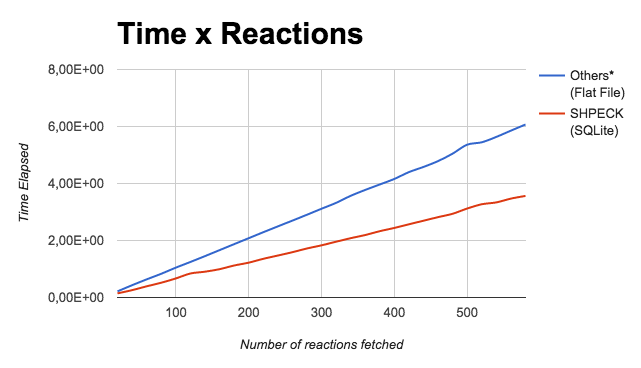
\includegraphics[width=140mm]{timeXreactionAccess.png}
\caption{Time elapsed in seconds X Reactions Accessed}
\label{fig:timeXaccess}
\end{figure}

\section{Concluding remarks}
This work provides details of \emph{SHPECK}, a modeling software package intended to raise the quality of available geochemical speciation. \emph{SHPECK} calculates the distribution of dissolved solutes in the water and saturation indices of various mineral phases. \emph{SHPECK} calculates the speciation of a solution based on a set of mass-balance equations, which are solved iteratively using the Newton-Raphson numerical method.

The program innovates by including a visual user interface that allows users to parametrize simulation configuration and input, as well as by using a relational database architecture component. The user interface implements a dynamic tool that facilitates the simulation case preparation. \emph{SHPECK} accepts any general combination of chemical elements, mineral species and chemical reactions, along with definitions of boundary contour conditions of temperature, pH, pressure, etc.

The software was tested and its results compared with those obtained by modeling the same study case with other geochemical modeling software. The results produced by \emph{SHPECK} were found to be consistent with those of the alternative models. All three alternative software evaluated produced nearly the same results. Slight differences were found when simulating with temperatures higher than $100^o$C, which appear to arise from discrepancies in how different software handle incomplete thermodynamic properties reactions.

We plan to improve \emph{SHPECK} by adding kinetic reactions to the processing core. The elemental mass evolution that will be required for the kinetic modeling involves mass change through mass transfer and kinetic reactions of solids and solute-solute interaction. The principles set forth in \cite{Ajpark:14} will be used.

We are also planning an implementation of a procedure for distributing \emph{SHPECK} from an Internet platform where users can register, download \emph{SHPECK}, interact, and collaborate in forums.

\section*{Acknowledgements}
This work has been supported by PETROBRAS, CNPq and CAPES. We also acknowledge the infrastructure provide by the Informatics Institute, specially the Centro de Empreendimentos em Informática (CEI), Federal University of Rio Grande do Sul, Brazil.


%% References
%%
%% Following citation commands can be used in the body text:
%% Usage of \cite is as follows:
%%   \cite{key}         ==>>  [#]
%%   \cite[chap. 2]{key} ==>> [#, chap. 2]
%%

%% References with bibTeX database:
\newpage
%\bibliographystyle{elsarticle-num}
% \bibliographystyle{elsarticle-harv}
 \bibliographystyle{abntex2-alf}
% \bibliographystyle{model1a-num-names}
% \bibliographystyle{model1b-num-names}
% \bibliographystyle{model1c-num-names}
% \bibliographystyle{model1-num-names}
% \bibliographystyle{model2-names}
% \bibliographystyle{model3a-num-names}
% \bibliographystyle{model3-num-names}
% \bibliographystyle{model4-names}
% \bibliographystyle{model5-names}
% \bibliographystyle{model6-num-names}

\bibliography{ref}


\end{document}

%%
%% End of file `elsarticle-template-num.tex'.
